\section{Synchronous machines}

%%%%%%%%%%%%%%%%%%%%%%%%%%%%%%%%%%%%%%%%%%%%%%%%%%%%%%%%%%%%%
\subsection{Operation principle and application examples}
%%%%%%%%%%%%%%%%%%%%%%%%%%%%%%%%%%%%%%%%%%%%%%%%%%%%%%%%%%%%%

%%%%%%%%%%%%%%%%%%%%%%%%%%%%%%%%%%%%%%%%%%%%%%%%%%%%%%%%%%%%%
%% Synchronous machine (SM) rotor types %%
%%%%%%%%%%%%%%%%%%%%%%%%%%%%%%%%%%%%%%%%%%%%%%%%%%%%%%%%%%%%%
\begin{frame}
	\frametitle{Synchronous machine (SM) rotor types}
	\begin{figure}
		\centering
		\begin{subfigure}{0.49\textwidth}
			\centering
			\includegraphics[width=0.8\textwidth]{fig/lec07/SM_salient_pole.pdf}
			\caption{Salient pole rotor}
		\end{subfigure}
		\hfill
		\begin{subfigure}{0.49\textwidth}
			\centering
			\includegraphics[width=0.8\textwidth]{fig/lec07/SM_cylindrical_rotor.pdf}
			\caption{Cylindrical rotor}
		\end{subfigure}
        \caption{Major rotor types of synchronous machines (SM)} 
        \label{fig:examples_SM_rotor}
	\end{figure}
\end{frame}

%%%%%%%%%%%%%%%%%%%%%%%%%%%%%%%%%%%%%%%%%%%%%%%%%%%%%%%%%%%%%
%% SM application examples %%
%%%%%%%%%%%%%%%%%%%%%%%%%%%%%%%%%%%%%%%%%%%%%%%%%%%%%%%%%%%%%
\begin{frame}
	\frametitle{SM application examples}
	\begin{figure}
		\centering
		\begin{subfigure}{0.49\textwidth}
			\centering
			\includegraphics[height=0.55\textheight]{fig/lec07/Salient_pole_rotor.jpg}
			\caption{\SI{2}{\mega\volt\ampere} generator from 1920 (source: \href{hhttps://commons.wikimedia.org/wiki/File:Drehstrom-Synchron-Generator.jpg}{Wikimedia Commons}, Kolossos, \href{https://creativecommons.org/licenses/by-sa/3.0/deed}{CC BY-SA 3.0})}
		\end{subfigure}
		\hfill
		\begin{subfigure}{0.49\textwidth}
			\centering
			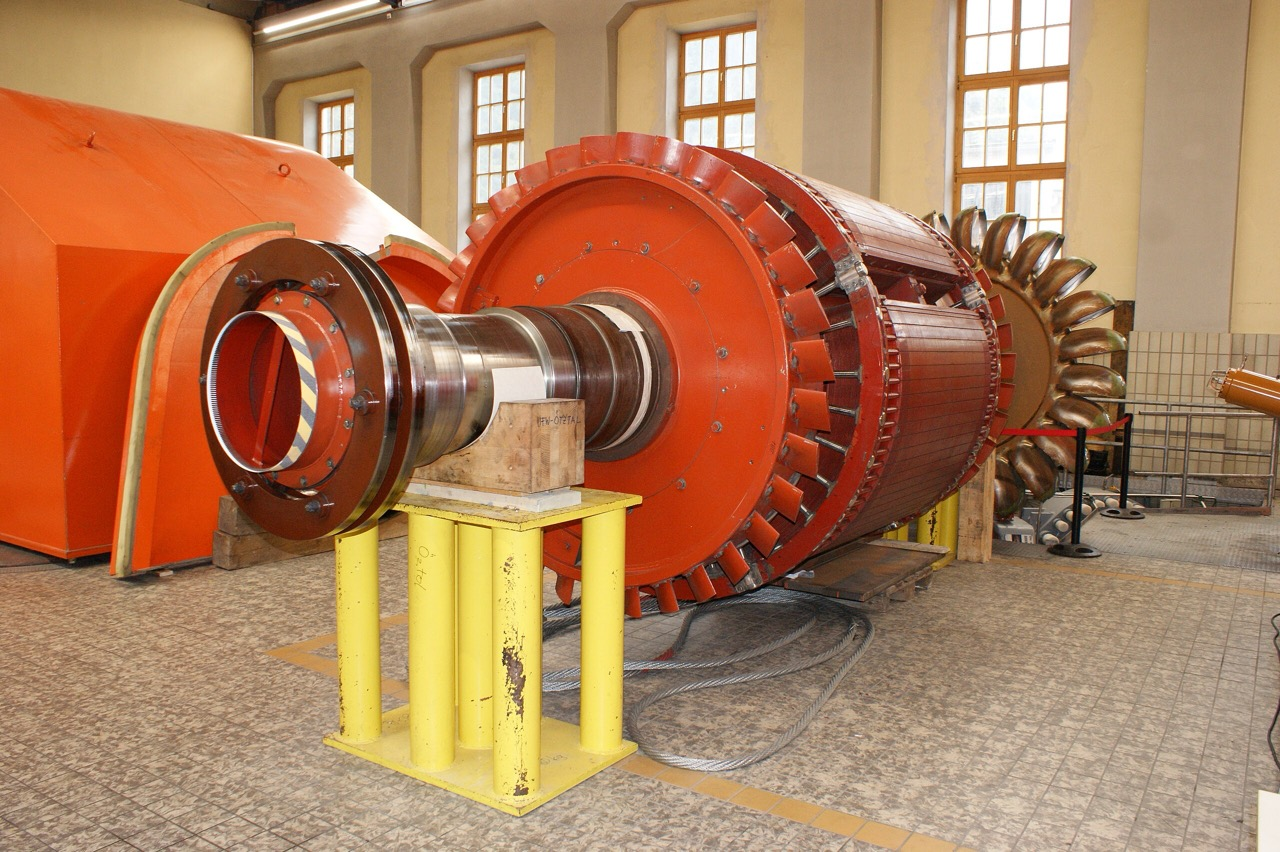
\includegraphics[height=0.55\textheight]{fig/lec07/Pelton_wheel_rotor.jpg}
			\caption{\SI[tight-spacing=true]{36}{\mega\volt\ampere} Pelton wheel generator (source: \href{https://commons.wikimedia.org/wiki/File:Wald_am_Arlberg-OeBB_Spullersee_power_plant-M1-Rotor-09ASD.jpg}{Wikimedia Commons},  	Asurnipal, \href{https://creativecommons.org/licenses/by-sa/4.0/deed}{CC BY-SA 4.0})} 
		\end{subfigure}
        \caption{SM examples with salient pole rotor type} 
        \label{fig:examples_SM_applications_01}
	\end{figure}
\end{frame}

%%%%%%%%%%%%%%%%%%%%%%%%%%%%%%%%%%%%%%%%%%%%%%%%%%%%%%%%%%%%%
%% SM application examples (cont.) %%
%%%%%%%%%%%%%%%%%%%%%%%%%%%%%%%%%%%%%%%%%%%%%%%%%%%%%%%%%%%%%
\begin{frame}
	\frametitle{SM application examples (cont.)}
	\begin{figure}
		\centering
		\begin{subfigure}{0.49\textwidth}
			\centering
			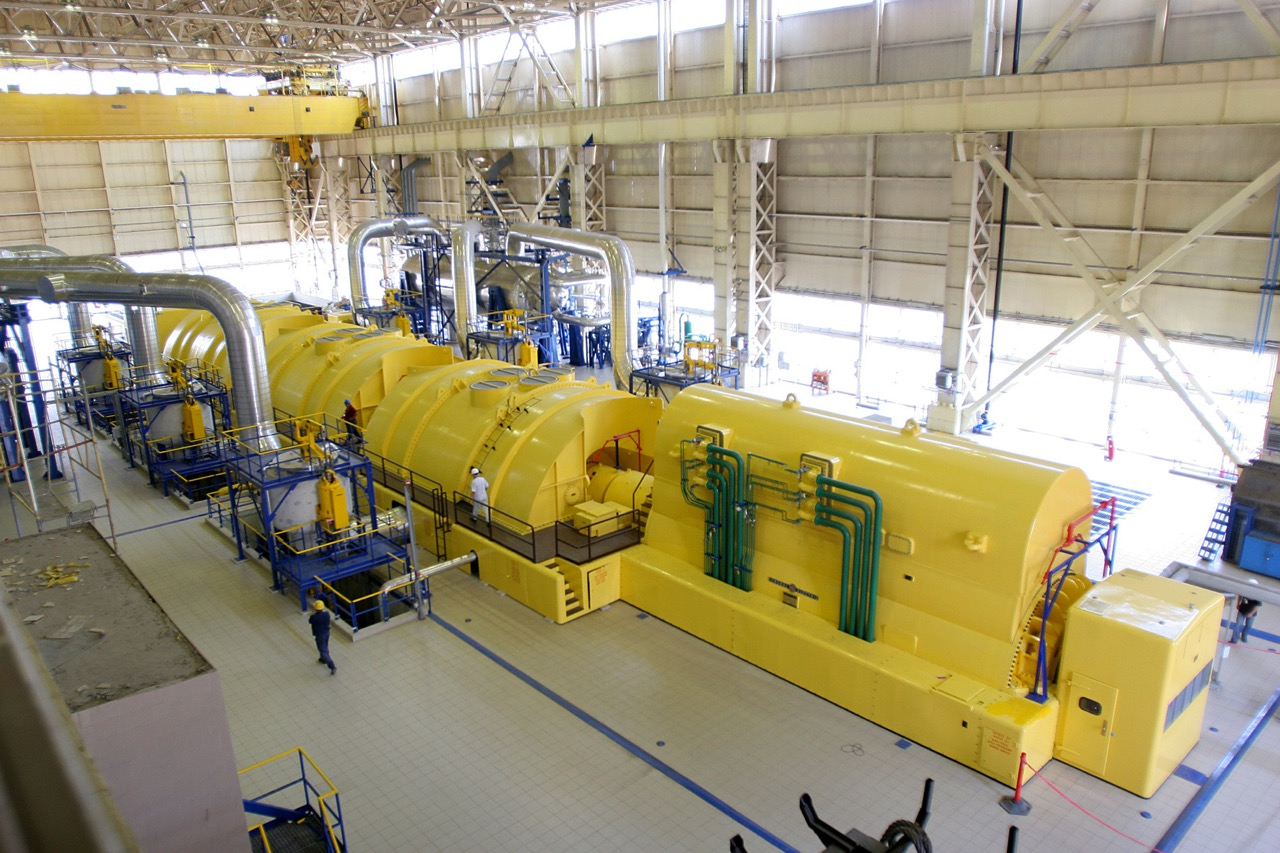
\includegraphics[height=0.55\textheight]{fig/lec07/Turbogenerator.jpg}
			\caption{\SI{650}{\mega\volt\ampere} turbogenerator from Cernavodă nuclear power plant (source: \href{https://commons.wikimedia.org/wiki/File:Grupul_turbogenerator_CNE_Cernavoda.jpg}{Wikimedia Commons}, R. Lavinia, \href{https://creativecommons.org/licenses/by-sa/4.0/deed}{CC BY-SA 4.0})}
		\end{subfigure}
		\hfill
		\begin{subfigure}{0.49\textwidth}
			\centering
			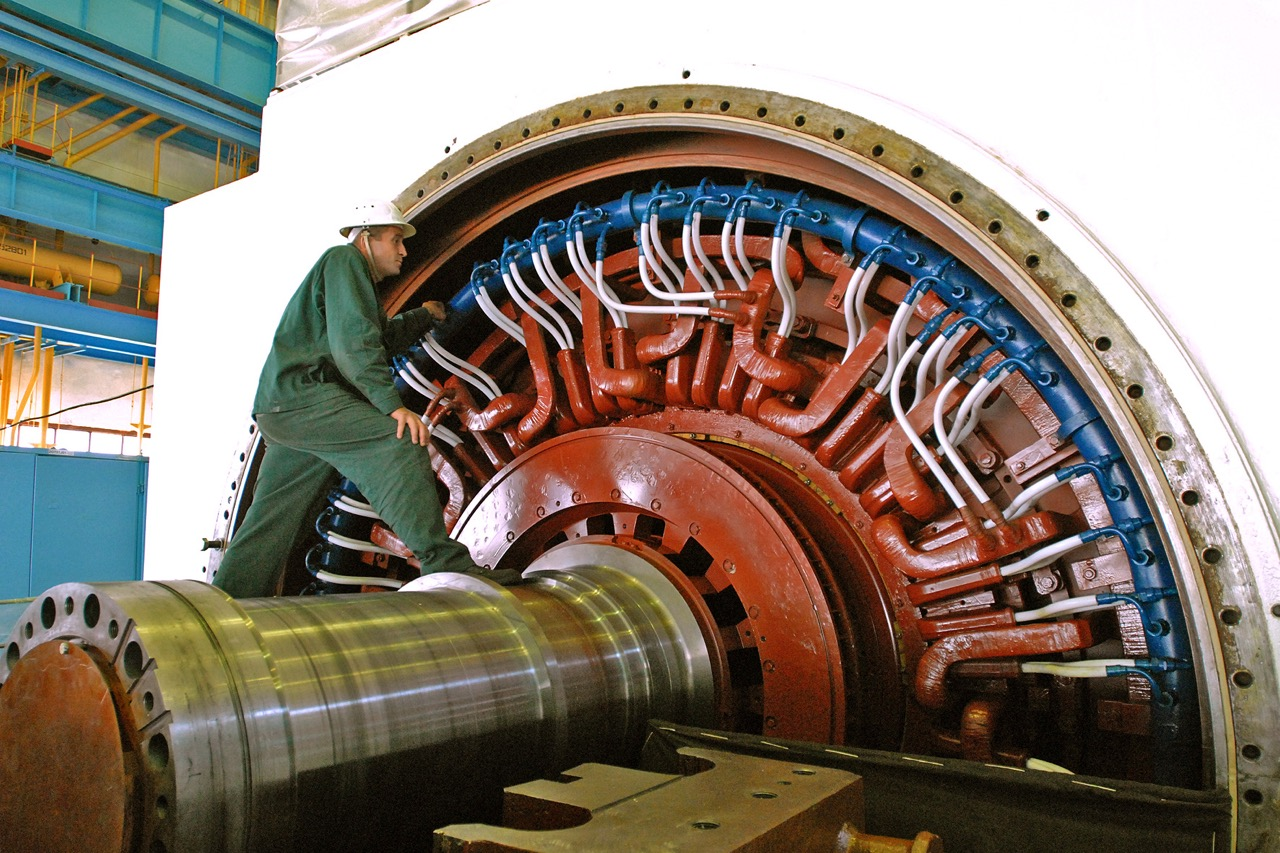
\includegraphics[height=0.55\textheight]{fig/lec07/Turbogenerator_rotor.jpg}
			\caption{\SI[tight-spacing=true]{1}{\giga\volt\ampere} turbogenerator SM rotor from Balakovo nuclear power plant (source: \href{https://commons.wikimedia.org/wiki/File:BalakovoNPP_tb.jpg}{Wikimedia Commons},  A. Seetenky, \href{https://creativecommons.org/licenses/by-sa/3.0/deed}{CC BY-SA 3.0})} 
		\end{subfigure}
        \caption{SM examples with cylindrical rotor type} 
        \label{fig:examples_SM_applications_02}
	\end{figure}
\end{frame}

%%%%%%%%%%%%%%%%%%%%%%%%%%%%%%%%%%%%%%%%%%%%%%%%%%%%%%%%%%%%%
%% Visualization of the synchronous machine operation %%
%%%%%%%%%%%%%%%%%%%%%%%%%%%%%%%%%%%%%%%%%%%%%%%%%%%%%%%%%%%%%
\begin{frame}
	\frametitle{Visualization of the synchronous machine operation}
    \begin{figure}
        \centering
        \movie{\includegraphics[height=0.85\textheight]{fig/lec07/SM_load_angle_90_preview.png}}{fig/lec07/SM_load_angle_90_animation.gif}
        \vspace{-0.25cm}
        \caption{Exemplary SM operation at $\omega=2 \pi \SI{50}{\per\second}$ in motoric operation (positive average torque)}
        \label{fig:SM_load_angle_90_animation}
    \end{figure}
\end{frame}

%%%%%%%%%%%%%%%%%%%%%%%%%%%%%%%%%%%%%%%%%%%%%%%%%%%%%%%%%%%%%
%% Visualization of the synchronous machine operation (cont.) %%
%%%%%%%%%%%%%%%%%%%%%%%%%%%%%%%%%%%%%%%%%%%%%%%%%%%%%%%%%%%%%
\begin{frame}
	\frametitle{Visualization of the synchronous machine operation (cont.)}
    \begin{figure}
        \centering
        \movie{\includegraphics[height=0.85\textheight]{fig/lec07/SM_load_angle_0_preview.png}}{fig/lec07/SM_load_angle_0_animation.gif}
        \vspace{-0.25cm}
        \caption{Exemplary SM operation at $\omega=2 \pi \SI{50}{\per\second}$ in no-load operation (zero average torque)}
        \label{fig:SM_load_angle_0_animation}
    \end{figure}
\end{frame}

%%%%%%%%%%%%%%%%%%%%%%%%%%%%%%%%%%%%%%%%%%%%%%%%%%%%%%%%%%%%%
\subsection{Model in stationary three-phase coordinates}
%%%%%%%%%%%%%%%%%%%%%%%%%%%%%%%%%%%%%%%%%%%%%%%%%%%%%%%%%%%%%

%%%%%%%%%%%%%%%%%%%%%%%%%%%%%%%%%%%%%%%%%%%%%%%%%%%%%%%%%%%%%
%% Dynamical IM model %%
%%%%%%%%%%%%%%%%%%%%%%%%%%%%%%%%%%%%%%%%%%%%%%%%%%%%%%%%%%%%%
\begin{frame}
	\frametitle{Dynamical SM model}
    Based on Faraday's and Ohm's laws, we can write the following equations for the stator 
    \begin{equation}
            \bm{u}^\mathrm{s}_\mathrm{s,abc}(t) = R_\mathrm{s}\bm{i}^\mathrm{s}_\mathrm{s,abc}(t)+\frac{\mathrm{d}}{\mathrm{d}t}\bm{\psi}^\mathrm{s}_\mathrm{s,abc}(t) \hspace{0.2cm} \Leftrightarrow \hspace{0.2cm} \begin{bmatrix}
                u_{\mathrm{s,a}}^\mathrm{s}(t)\\
                u_{\mathrm{s,b}}^\mathrm{s}(t)\\
                u_{\mathrm{s,c}}(t)\\
            \end{bmatrix} = R_\mathrm{s} \begin{bmatrix}
                i_{\mathrm{s,a}}^\mathrm{s}(t)\\
                i_{\mathrm{s,b}}^\mathrm{s}(t)\\
                i_{\mathrm{s,c}}^\mathrm{s}(t)\\
            \end{bmatrix} + \frac{\mathrm{d}}{\mathrm{d}t} \begin{bmatrix}
                \psi_{\mathrm{s,a}}^\mathrm{s}(t)\\
                \psi_{\mathrm{s,b}}^\mathrm{s}(t)\\
                \psi_{\mathrm{s,c}}^\mathrm{s}(t)\\
            \end{bmatrix}
            \label{eq:SM_stator_three_phase_voltage_equation}
    \end{equation}
    \pause
    and rotor field winding
    \begin{equation}
            u^\mathrm{r}_\mathrm{f}(t) = R_\mathrm{f}i^\mathrm{r}_\mathrm{f}(t)+\frac{\mathrm{d}}{\mathrm{d}t}\psi^\mathrm{r}_\mathrm{f}(t) 
            \label{eq:SM_rotor_voltage_equation}
    \end{equation}
which are generally applicable as only identical resistances per phase on the stator are assumed. \pause In contrast to the induction motor, only a single rotor field winding is present.
\end{frame}

%%%%%%%%%%%%%%%%%%%%%%%%%%%%%%%%%%%%%%%%%%%%%%%%%%%%%%%%%%%%%
%% Flux linakge model %%
%%%%%%%%%%%%%%%%%%%%%%%%%%%%%%%%%%%%%%%%%%%%%%%%%%%%%%%%%%%%%
\begin{frame}
	\frametitle{Flux linkage model}
    \onslide<2->
    \begin{columns}
		\begin{column}{0.55\textwidth}
			The SM flux linkage model is similar to the IM model:
	       \begin{itemize}
            \item<2-> Assuming a cylindrical rotor, the self-induced stator flux remains identical to the IM model (derived from rotating field theory chapter).
            \item<3-> In contrast to the IM model \figref{fig:Inductive_coupling_stator_rotor_IM}, the SM's rotor field coil is a represented by a single winding. 
            \item<4-> The coupling of the stator and rotor remains rotor position-dependent (not explicitly shown on the right due to space limitations). 
           \end{itemize}
        \end{column}
        \begin{column}{0.45\textwidth}
            \onslide<1->
                \begin{figure}
                    \centering
                    \includegraphics[width=0.75\textwidth]{fig/lec07/Inductive_coupling_stator_rotor.pdf}
                    \caption{Simplified representation of the inductive coupling between the stator/rotor phases of the cylindrical rotor SM}
                    \label{fig:Inductive_coupling_stator_rotor_SM}
                \end{figure}
        \end{column}
    \end{columns}
\end{frame}

%%%%%%%%%%%%%%%%%%%%%%%%%%%%%%%%%%%%%%%%%%%%%%%%%%%%%%%%%%%%%
%% Flux linakge model %%
%%%%%%%%%%%%%%%%%%%%%%%%%%%%%%%%%%%%%%%%%%%%%%%%%%%%%%%%%%%%%
\begin{frame}
	\frametitle{Flux linkages of the three-phase model}
    \onslide<1->
    Based on the previous considerations, the flux linkages of the cylindrical SM are given by
    \begin{equation}
        \renewcommand*{\arraystretch}{1.15}
        \begin{split}
            \uncover<+->{
            \bm{\psi}^\mathrm{s}_\mathrm{s,abc}(t) &=\begin{bmatrix}
                L_\mathrm{s} & -\frac{M_\mathrm{s}}{2} & -\frac{M_\mathrm{s}}{2}\\
                -\frac{M_\mathrm{s}}{2} & L_\mathrm{s} & -\frac{M_\mathrm{s}}{2}\\
                -\frac{M_\mathrm{s}}{2} & -\frac{M_\mathrm{s}}{2} & L_\mathrm{s}
            \end{bmatrix} \bm{i}^\mathrm{s}_\mathrm{s,abc}(t)}\uncover<+->{ +  M_{\mathrm{r}}\frac{N_\mathrm{s}}{N_\mathrm{r}} \begin{bmatrix}
				\cos(\varepsilon_\mathrm{r,el}(t))\\
				 \cos(\varepsilon_\mathrm{r,el}(t) - \frac{2\pi}{3})\\
				 \cos(\varepsilon_\mathrm{r,el}(t) + \frac{2\pi}{3}) 
			 \end{bmatrix}i^\mathrm{r}_\mathrm{f}(t),}\\
            \uncover<+->{
            \psi^\mathrm{r}_\mathrm{f}(t) &= L_\mathrm{f} i^\mathrm{r}_\mathrm{f}(t)\\ &+  M_{\mathrm{s}}\frac{N_\mathrm{r}}{N_\mathrm{s}} \begin{bmatrix}
				\cos(\varepsilon_\mathrm{r,el}(t))  & \cos(\varepsilon_\mathrm{r,el}(t) - \frac{2\pi}{3}) & \cos(\varepsilon_\mathrm{r,el}(t) + \frac{2\pi}{3}) 
			 \end{bmatrix}\bm{i}^\mathrm{s}_\mathrm{s,abc}(t)}
        \end{split}
        \label{eq:Flux_linkage_model_SM_abc}
    \end{equation}
	\onslide<+-> 
    with $\varepsilon_\mathrm{r,el}(t)=p\varepsilon_\mathrm{r}(t)$. \onslide<+-> Consequently, \eqref{eq:Flux_linkage_model_SM_abc} can be interpreted as a reduced representation of the IM's flux linkage model \eqref{eq:Flux_linkage_model_IM_abc}.
\end{frame}

%%%%%%%%%%%%%%%%%%%%%%%%%%%%%%%%%%%%%%%%%%%%%%%%%%%%%%%%%%%%%
\subsection{Model in stationary alpha-beta coordinates}
%%%%%%%%%%%%%%%%%%%%%%%%%%%%%%%%%%%%%%%%%%%%%%%%%%%%%%%%%%%%%

%%%%%%%%%%%%%%%%%%%%%%%%%%%%%%%%%%%%%%%%%%%%%%%%%%%%%%%%%%%%%
%% Cylindrical SM model in alpha-beta coordinates: voltage equations %%
%%%%%%%%%%%%%%%%%%%%%%%%%%%%%%%%%%%%%%%%%%%%%%%%%%%%%%%%%%%%%
\begin{frame}
	\frametitle{Cylindrical SM model in alpha-beta coordinates: voltage equations}
    \begin{columns}
		\begin{column}{0.55\textwidth}
	       Similar to the IM, we can represent the SM model is orthogonal $\alpha\beta$-coordinates. For the SM this only applies to the three-phase stator, as the rotor has only a single phase winding. The $\alpha\beta$-coordinates voltage equation is given by (compare to \eqref{eq:IM_stator_alpha_beta_voltage_equation})
		   \begin{equation}
			\bm{u}^\mathrm{s}_\mathrm{s,\alpha\beta}(t) = R_\mathrm{s} \bm{i}^\mathrm{s}_\mathrm{s,\alpha\beta}(t)+ \frac{\mathrm{d}}{\mathrm{d}t}\bm{\psi}^\mathrm{s}_\mathrm{s,\alpha\beta}(t)
		   \end{equation}
		   \onslide<2->
		   while the rotor field winding voltage equation remains identical to \eqref{eq:SM_rotor_voltage_equation}:
		   $$
			u^\mathrm{r}_\mathrm{f}(t) = R_\mathrm{f}i^\mathrm{r}_\mathrm{f}(t)+\frac{\mathrm{d}}{\mathrm{d}t}\psi^\mathrm{r}_\mathrm{f}(t).
			$$
        \end{column}
        \begin{column}{0.45\textwidth}
            \onslide<1->
            \begin{figure}
                \centering
                \includegraphics[width=0.85\textwidth]{fig/lec07/SM_cylindrical_rotor_alpha_beta.pdf}
                \caption{Conceptual cylindrical SM representation within the orthogonal $\alpha\beta$ coordinates ($p=1$ pole pair)}
                \label{fig:SM_alpha_beta}
            \end{figure}
        \end{column}
    \end{columns}
\end{frame}


%%%%%%%%%%%%%%%%%%%%%%%%%%%%%%%%%%%%%%%%%%%%%%%%%%%%%%%%%%%%%
%% Cylindrical SM model in alpha-beta coordinates: flux linkage %%
%%%%%%%%%%%%%%%%%%%%%%%%%%%%%%%%%%%%%%%%%%%%%%%%%%%%%%%%%%%%%
\begin{frame}
	\frametitle{Cylindrical SM model in alpha-beta coordinates: flux linkage}
	\onslide<+->
	For the flux linkage model in $\alpha\beta$-coordinates, we multiply the stator flux equations from \eqref{eq:Flux_linkage_model_SM_abc} with $\bm{T}_{23}$ from the right
	\begin{equation}
		\begin{split}
			\uncover<+->{
			\bm{\psi}^\mathrm{s}_\mathrm{s,\alpha\beta}(t)  &= \bm{T}_{23} \bm{\psi}^\mathrm{s}_\mathrm{s,abc}(t) = \overbrace{\bm{T}_{23} \bm{L}_{\mathrm{s,abc}}\bm{T}_{32}}^{\bm{L}_{\mathrm{s},\alpha\beta}} \bm{i}^\mathrm{s}_{\mathrm{s},\alpha\beta}(t) +  M_{\mathrm{r}}\frac{N_\mathrm{s}}{N_\mathrm{r}} \bm{T}_{23}\begin{bmatrix}
				\cos(\varepsilon_\mathrm{r,el}(t))\\
				 \cos(\varepsilon_\mathrm{r,el}(t) - \frac{2\pi}{3})\\
				 \cos(\varepsilon_\mathrm{r,el}(t) + \frac{2\pi}{3}) 
			 \end{bmatrix} i^\mathrm{r}_{\mathrm{f}}(t)\\}
			 \uncover<+->{& = (L_\mathrm{s} +\nicefrac{M_\mathrm{s}}{2}) \bm{i}^\mathrm{s}_{\mathrm{s},\alpha\beta}(t) + M_\mathrm{r}\frac{N_\mathrm{s}}{N_\mathrm{r}} \begin{bmatrix}\cos(\varepsilon_\mathrm{r,el}(t))\\ \sin(\varepsilon_\mathrm{r,el}(t))\end{bmatrix} i^\mathrm{r}_{\mathrm{f}}(t)}
			\end{split}
	\end{equation}
	\onslide<+->
	and utilize $\bm{i}^\mathrm{s}_\mathrm{s,abc}(t)=\bm{T}_{32} \bm{i}^\mathrm{s}_\mathrm{s,\alpha\beta}(t)$ to modify the rotor flux linkage equation accordingly:
	\begin{equation}
		\begin{split}
			\psi^\mathrm{r}_\mathrm{f}(t) &= L_\mathrm{f} i^\mathrm{r}_\mathrm{f}(t) + M_{\mathrm{s}}\frac{N_\mathrm{r}}{N_\mathrm{s}} \begin{bmatrix}
				\cos(\varepsilon_\mathrm{r,el}(t))  & \sin(\varepsilon_\mathrm{r,el}(t))
			 \end{bmatrix}\bm{i}^\mathrm{s}_\mathrm{s,\alpha\beta}(t).
		\end{split}
	\end{equation} 
	\onslide<+->
	In contrast to the IM $\alpha\beta$-coordinates flux linkage model, the SM flux-to-current coupling is rotor position-dependent.
\end{frame}

%%%%%%%%%%%%%%%%%%%%%%%%%%%%%%%%%%%%%%%%%%%%%%%%%%%%%%%%%%%%%
%% Cylindrical SM model in alpha-beta coordinates: flux linkage (cont.) %%
%%%%%%%%%%%%%%%%%%%%%%%%%%%%%%%%%%%%%%%%%%%%%%%%%%%%%%%%%%%%%
\begin{frame}
	\frametitle{Cylindrical SM model in alpha-beta coordinates: flux linkage (cont.)}
	\onslide<+->
	Analyzing the (magnetic) power balance reveals
    \begin{equation}
        M_\mathrm{r}\frac{N_\mathrm{s}}{N_\mathrm{r}} = M_{\mathrm{s}}\frac{N_\mathrm{r}}{N_\mathrm{s}} \stackrel{!}{=} M_\mathrm{fs}, 
    \end{equation}
	\onslide<+->
    and with the shorter notation 
		\begin{equation}
			L'_\mathrm{s} = (L_\mathrm{s} +\nicefrac{M_\mathrm{s}}{2})
		\end{equation}
	we can rewrite the flux linkage model in $\alpha\beta$-coordinates to
	\begin{equation}
		\begin{alignedat}{2}
			\uncover<+->{
			\bm{\psi}^\mathrm{s}_\mathrm{s,\alpha\beta}(t) &= L'_\mathrm{s} \bm{i}^\mathrm{s}_{\mathrm{s},\alpha\beta}(t) &&+ M_\mathrm{fs} \begin{bmatrix}\cos(\varepsilon_\mathrm{r,el}(t))\\ \sin(\varepsilon_\mathrm{r,el}(t))\end{bmatrix} i^\mathrm{r}_{\mathrm{f}}(t),\\}
			\uncover<+->{
			\psi^\mathrm{r}_\mathrm{f}(t) &= L_\mathrm{f} i^\mathrm{r}_\mathrm{f}(t) &&+ M_\mathrm{fs} \begin{bmatrix}\cos(\varepsilon_\mathrm{r,el}(t)) \\ \sin(\varepsilon_\mathrm{r,el}(t))\end{bmatrix}\T\bm{i}^\mathrm{s}_\mathrm{s,\alpha\beta}(t).}
		\end{alignedat}
		\label{eq:Flux_linkage_model_SM_alpha_beta}
	\end{equation}
\end{frame}

%%%%%%%%%%%%%%%%%%%%%%%%%%%%%%%%%%%%%%%%%%%%%%%%%%%%%%%%%%%%%
%% Cylindrical SM model in alpha-beta coordinates: torque %%
%%%%%%%%%%%%%%%%%%%%%%%%%%%%%%%%%%%%%%%%%%%%%%%%%%%%%%%%%%%%%
\begin{frame}
	\frametitle{Cylindrical SM model in alpha-beta coordinates: torque}
	\onslide<+->
	Following the same power balance approach as from the IM, the SM's torque equation is given by
	\begin{equation}
		T(t) = \frac{3}{2} p (\bm{i}_\mathrm{s,\alpha\beta}^\mathrm{s}(t))\T\bm{J}\bm{\psi}_\mathrm{s,\alpha\beta}^\mathrm{s}(t).
	\end{equation}
	\onslide<+->
	The equivalent representation with the rotor current and flux linkage as in the IM case is not applicable in the SM case, as the rotor has only a single field winding, i.e., is lacking an $\alpha\beta$ representation. \onslide<+-> Inserting the linear flux linkage model from \eqref{eq:Flux_linkage_model_SM_alpha_beta} into the torque equation yields
	\begin{equation}
		\begin{split}
			\uncover<+->{
			T(t) &= \frac{3}{2} p (\bm{i}_\mathrm{s,\alpha\beta}^\mathrm{s}(t))\T\bm{J}\bm{\psi}_\mathrm{s,\alpha\beta}^\mathrm{s}(t)\\}
			\uncover<+->{&= \frac{3}{2} p (\bm{i}_\mathrm{s,\alpha\beta}^\mathrm{s}(t))\T\bm{J}\left(L'_\mathrm{s} \bm{i}^\mathrm{s}_{\mathrm{s},\alpha\beta}(t) + M_\mathrm{fs} \begin{bmatrix}\cos(\varepsilon_\mathrm{r,el}(t))\\ \sin(\varepsilon_\mathrm{r,el}(t))\end{bmatrix} i^\mathrm{r}_{\mathrm{f}}(t)\right)\\}
			\uncover<+->{&= \frac{3}{2} p M_\mathrm{fs} i^\mathrm{r}_{\mathrm{f}} \left(\cos(\varepsilon_\mathrm{r,el}(t))i_{\mathrm{s,\beta}}^\mathrm{s}(t) - \sin(\varepsilon_\mathrm{r,el}(t))i_{\mathrm{s,\alpha}}^\mathrm{s}(t)\right).}
		\end{split}
		\label{eq:SM_cylindrical_alphabeta_torque_equation}
	\end{equation}
\end{frame}


%%%%%%%%%%%%%%%%%%%%%%%%%%%%%%%%%%%%%%%%%%%%%%%%%%%%%%%%%%%%%
%% Cylindrical SM model in alpha-beta coordinates: voltage equations %%
%%%%%%%%%%%%%%%%%%%%%%%%%%%%%%%%%%%%%%%%%%%%%%%%%%%%%%%%%%%%%
\begin{frame}
	\frametitle{Cylindrical SM model in alpha-beta coordinates: torque interpretation}
    \begin{columns}
		\begin{column}{0.55\textwidth}
			\onslide<+->
			In \eqref{eq:SM_cylindrical_alphabeta_torque_equation} the term
			\begin{equation}
				M_\mathrm{fs} \begin{bmatrix}\cos(\varepsilon_\mathrm{r,el}(t))\\ \sin(\varepsilon_\mathrm{r,el}(t))\end{bmatrix} i^\mathrm{r}_{\mathrm{f}}(t) =\bm{\psi}^\mathrm{s}_{\mathrm{f}}(t)
			\end{equation}
			can be interpreted as the field winding flux linkage coupled with the stator winding. \onslide<+-> Hence, the torque expression can be rewritten as:
			\begin{equation}
				\begin{split}
				T(t) &= \frac{3}{2} p \left\|\bm{\psi}^\mathrm{s}_{\mathrm{f}}(t) \times \bm{i}^\mathrm{s}_{\mathrm{s,\alpha\beta}}(t)\right\| \\ &= \frac{3}{2} p \left\|\bm{\psi}^\mathrm{s}_{\mathrm{f}}(t) \vphantom{\bm{i}^\mathrm{s}_{\mathrm{s,\alpha\beta}}(t)}\right\| \left\| \bm{i}^\mathrm{s}_{\mathrm{s,\alpha\beta}}(t)\right\| \sin(\theta(t))
			\end{split}
			\end{equation}
			with $\theta$ being the angle between the field winding flux linkage and the stator current vectors, also known as the load angle.
        \end{column}
        \begin{column}{0.45\textwidth}
            \onslide<3->
            \begin{figure}
                \centering
                \includegraphics[width=0.75\textwidth]{fig/lec07/Torque_interpretation.pdf}
                \caption{Interpretation of the torque as the parallelogram area spannend by the vectors of the field winding flux and the stator current}
                \label{fig:Torque_interpretation}
            \end{figure}
        \end{column}
    \end{columns}
\end{frame}

%%%%%%%%%%%%%%%%%%%%%%%%%%%%%%%%%%%%%%%%%%%%%%%%%%%%%%%%%%%%%
%% Summary: cylindrical SM model in $\alpha\beta$ coordinates   %%
%%%%%%%%%%%%%%%%%%%%%%%%%%%%%%%%%%%%%%%%%%%%%%%%%%%%%%%%%%%%%
\begin{frame}
	\frametitle{Summary: cylindrical SM model in $\alpha\beta$ coordinates}
    The most important equations of the cylindrical SM model in the  $\alpha\beta$ coordinates are:
    \begin{equation*}
        \begin{alignedat}{4}
            &&\mbox{Stator voltage:}&& \quad\bm{u}^\mathrm{s}_\mathrm{s,\alpha\beta}(&t) &&= R_\mathrm{s} \bm{i}^\mathrm{s}_\mathrm{s,\alpha\beta}(t)+ \frac{\mathrm{d}}{\mathrm{d}t}\bm{\psi}^\mathrm{s}_\mathrm{s,\alpha\beta}(t),\\
            &&\mbox{Rotor / field winding voltage:}&& \quad u^\mathrm{r}_\mathrm{f}(&t) &&= R_\mathrm{f}i^\mathrm{r}_\mathrm{f}(t)+\frac{\mathrm{d}}{\mathrm{d}t}\psi^\mathrm{r}_\mathrm{f}(t),\\
            &&\mbox{Stator flux linkage:}&& \quad \bm{\psi}^\mathrm{s}_\mathrm{s,\alpha\beta}(&t) &&= L'_\mathrm{s} \bm{i}^\mathrm{s}_{\mathrm{s},\alpha\beta}(t) + M_\mathrm{fs} \begin{bmatrix}\cos(\varepsilon_\mathrm{r,el}(t))\\ \sin(\varepsilon_\mathrm{r,el}(t))\end{bmatrix} i^\mathrm{r}_{\mathrm{f}}(t),\\
            &&\mbox{Rotor / field winding flux linkage:}&& \psi^\mathrm{r}_\mathrm{f}(&t) &&= L_\mathrm{f} i^\mathrm{r}_\mathrm{f}(t) + M_\mathrm{fs} \begin{bmatrix}\cos(\varepsilon_\mathrm{r,el}(t)) \\ \sin(\varepsilon_\mathrm{r,el}(t))\end{bmatrix}\T\bm{i}^\mathrm{s}_\mathrm{s,\alpha\beta}(t),\\
            &&\mbox{Torque:}&& \quad T(&t) &&= \frac{3}{2} p (\bm{i}_\mathrm{s,\alpha\beta}^\mathrm{s})\T\bm{J}\bm{\psi}_\mathrm{s,\alpha\beta}^\mathrm{s}. 
        \end{alignedat}
    \end{equation*}
\end{frame}

%%%%%%%%%%%%%%%%%%%%%%%%%%%%%%%%%%%%%%%%%%%%%%%%%%%%%%%%%%%%%
\subsection{Model in rotary d-q coordinates}
%%%%%%%%%%%%%%%%%%%%%%%%%%%%%%%%%%%%%%%%%%%%%%%%%%%%%%%%%%%%%

%%%%%%%%%%%%%%%%%%%%%%%%%%%%%%%%%%%%%%%%%%%%%%%%%%%%%%%%%%%%%
%% Rotor flux orientation: the dq coordinate system %%
%%%%%%%%%%%%%%%%%%%%%%%%%%%%%%%%%%%%%%%%%%%%%%%%%%%%%%%%%%%%%
\begin{frame}
	\frametitle{Rotor flux orientation: the dq coordinate system}	
    \begin{columns}
		\begin{column}{0.5\textwidth}
			\begin{itemize}
				\item In the SM case the rotor flux orientaton is directly related to the rotor position (cf. \figref{fig:examples_SM_rotor}). 
				\item Hence, to transfer the rotor and stator equations into a mutual coordinate system, the rotor flux orientation is typically used as a reference. 
				\item In contrast to the $\alpha\beta$-coordinates, where the stator quantity signals are of sinusoidal shape during steady state, the rotor flux-oriented signals are constant during steady state.
			\end{itemize}
		\end{column}
        \begin{column}{0.5\textwidth}
            \begin{figure}
                \centering
                \includegraphics[width=0.9\textwidth]{fig/lec07/dq_orientation.pdf}
                \caption{Rotor flux-oriented coordinate system}
                \label{fig:dq_orientation}
            \end{figure}
        \end{column}
    \end{columns}
\end{frame}

%%%%%%%%%%%%%%%%%%%%%%%%%%%%%%%%%%%%%%%%%%%%%%%%%%%%%%%%%%%%%
%% Rotor flux orientation: the dq coordinate system (cont.) %%
%%%%%%%%%%%%%%%%%%%%%%%%%%%%%%%%%%%%%%%%%%%%%%%%%%%%%%%%%%%%%
\begin{frame}
	\frametitle{Rotor flux orientation: the dq coordinate system (cont.) }
	\onslide<1->
	Transferring the stator voltage equation into the dq coordinate system results in
		   \begin{equation}
			\begin{split}
			\uncover<+->{
			\bm{u}^\mathrm{s}_\mathrm{s,\alpha\beta}(t) &= R_\mathrm{s} \bm{i}^\mathrm{s}_\mathrm{s,\alpha\beta}(t)+ \frac{\mathrm{d}}{\mathrm{d}t}\bm{\psi}^\mathrm{s}_\mathrm{s,\alpha\beta}(t)\\}
			\uncover<+->{\Leftrightarrow \quad \bm{T}^{-1}_\mathrm{p}(\varepsilon_\mathrm{r,el})\bm{u}^\mathrm{s}_\mathrm{s,dq}(t) &= R_\mathrm{s} \bm{T}^{-1}_\mathrm{p}(\varepsilon_\mathrm{r,el})\bm{i}^\mathrm{s}_\mathrm{s,dq}(t)+ \frac{\mathrm{d}}{\mathrm{d}t}(\bm{T}^{-1}_\mathrm{p}(\varepsilon_\mathrm{r,el})\bm{\psi}^\mathrm{s}_\mathrm{s,dq}(t))\\}
			\uncover<+->{\Leftrightarrow \quad \bm{u}^\mathrm{r}_\mathrm{s,dq}(t) &= R_\mathrm{s} \bm{i}^\mathrm{r}_\mathrm{s,dq}(t)+ \omega_\mathrm{r,el}(t)\bm{J}\bm{\psi}^\mathrm{r}_\mathrm{s,dq}(t) + \frac{\mathrm{d}}{\mathrm{d}t}\bm{\psi}^\mathrm{r}_\mathrm{s,dq}(t).}
		\end{split}
		\end{equation}
		\onslide<+->
	Since the dq coordinate system is always aligned with the rotor flux in the SM case, one can also drop the superscript $\mathrm{r}$:
	\begin{equation*}
		\bm{u}_\mathrm{s,dq}(t) = R_\mathrm{s} \bm{i}_\mathrm{s,dq}(t)+ \omega_\mathrm{r,el}(t)\bm{J}\bm{\psi}_\mathrm{s,dq}(t) + \frac{\mathrm{d}}{\mathrm{d}t}\bm{\psi}_\mathrm{s,dq}(t).
	\end{equation*} 
\end{frame}

%%%%%%%%%%%%%%%%%%%%%%%%%%%%%%%%%%%%%%%%%%%%%%%%%%%%%%%%%%%%%
%% Rotor flux orientation: the dq coordinate system (cont.) %%
%%%%%%%%%%%%%%%%%%%%%%%%%%%%%%%%%%%%%%%%%%%%%%%%%%%%%%%%%%%%%
\begin{frame}
	\frametitle{Rotor flux orientation: the dq coordinate system (cont.) }
	\onslide<1->
	The stator flux linkage model in the dq coordinate system is given by
	\begin{equation}
		\begin{split}
			\uncover<+->{\bm{\psi}^\mathrm{s}_\mathrm{s,\alpha\beta}(t) &= L'_\mathrm{s} \bm{i}^\mathrm{s}_{\mathrm{s},\alpha\beta}(t) + M_\mathrm{fs} \begin{bmatrix}\cos(\varepsilon_\mathrm{r,el}(t))\\ \sin(\varepsilon_\mathrm{r,el}(t))\end{bmatrix} i^\mathrm{r}_{\mathrm{f}}(t),			 \\} 
			\uncover<+->{\Leftrightarrow \quad 
			 \bm{T}^{-1}_\mathrm{p}(\varepsilon_\mathrm{r,el}) \bm{\psi}_\mathrm{s,dq}(t) &= L'_\mathrm{s}  \bm{T}^{-1}_\mathrm{p}(\varepsilon_\mathrm{r,el})\bm{i}_{\mathrm{s, dq}}(t) + M_\mathrm{fs} \begin{bmatrix}\cos(\varepsilon_\mathrm{r,el}(t)) \\ \sin(\varepsilon_\mathrm{r,el}(t))\end{bmatrix}i_{\mathrm{f}}(t) \\}
			 \uncover<+->{\Leftrightarrow \quad \bm{\psi}_\mathrm{s,dq}(t) &= L'_\mathrm{s} \bm{i}_{\mathrm{s,dq}}(t) + \underbrace{M_\mathrm{fs} \begin{bmatrix}1 \\ 0 \end{bmatrix}}_{\bm{M}_\mathrm{fs}}i^\mathrm{r}_{\mathrm{f}}(t)} \uncover<+->{= L'_\mathrm{s} \bm{i}_{\mathrm{s,dq}}(t) + \bm{M}_\mathrm{fs}i^\mathrm{r}_{\mathrm{f}}(t).}
		\end{split}
		\label{eq:SM_stator_dq_flux_linkage}
	\end{equation}
	\onslide<5->
	while the field winding flux results in
	\begin{equation}
		\begin{split}
			\uncover<+->{\psi^\mathrm{r}_\mathrm{f}(t) &= L_\mathrm{f} i^\mathrm{r}_\mathrm{f}(t) + M_\mathrm{fs} \begin{bmatrix}\cos(\varepsilon_\mathrm{r,el}(t)) & \sin(\varepsilon_\mathrm{r,el}(t))\end{bmatrix}\bm{i}^\mathrm{s}_\mathrm{s,\alpha\beta}(t)
			 \\} 
			 \uncover<+->{\Leftrightarrow \quad 	 \psi^\mathrm{r}_\mathrm{f}(t) &= L_\mathrm{f} i^\mathrm{r}_\mathrm{f}(t) + M_\mathrm{fs} \begin{bmatrix}\cos(\varepsilon_\mathrm{r,el}(t)) & \sin(\varepsilon_\mathrm{r,el}(t))\end{bmatrix}  \bm{T}^{-1}_\mathrm{p}(\varepsilon_\mathrm{r,el})\bm{i}^\mathrm{s}_\mathrm{s,dq}(t)
			 \\}
			 \uncover<+->{\Leftrightarrow \quad \psi^\mathrm{r}_\mathrm{f}(t) &= L_\mathrm{f} i^\mathrm{r}_\mathrm{f}(t) + M_\mathrm{fs} \begin{bmatrix}1 & 0\end{bmatrix} \bm{i}_\mathrm{s,dq}(t)}\uncover<+->{= L_\mathrm{f} i^\mathrm{r}_\mathrm{f}(t) + \bm{M}\T_\mathrm{fs} \bm{i}_\mathrm{s,dq}(t).}
		\end{split}
	\end{equation}
\end{frame}

%%%%%%%%%%%%%%%%%%%%%%%%%%%%%%%%%%%%%%%%%%%%%%%%%%%%%%%%%%%%%
%% Summary: Cylindrical SM model in dq coordinates   %%
%%%%%%%%%%%%%%%%%%%%%%%%%%%%%%%%%%%%%%%%%%%%%%%%%%%%%%%%%%%%%
\begin{frame}
	\frametitle{Summary: cylindrical SM model in dq coordinates}
    The most important equations of the cylindrical SM model in the  dq coordinates are:
    \begin{equation*}
        \begin{alignedat}{4}
            &&\mbox{Stator voltage:}&& \quad\bm{u}_\mathrm{s,dq}(&t) &&= R_\mathrm{s} \bm{i}_\mathrm{s,dq}(t)+ \omega_\mathrm{r,el}(t)\bm{J}\bm{\psi}_\mathrm{s,dq}(t) + \frac{\mathrm{d}}{\mathrm{d}t}\bm{\psi}_\mathrm{s,dq}(t),\\
			&&\mbox{Rotor / field winding  voltage:}&& \quad u_\mathrm{f}(&t) &&= R_\mathrm{f}i_\mathrm{f}(t)+\frac{\mathrm{d}}{\mathrm{d}t}\psi_\mathrm{f}(t),\\
			&&\mbox{Stator flux linkage:}&& \quad \bm{\psi}_\mathrm{s,dq}(&t) &&= L'_\mathrm{s} \bm{i}_\mathrm{s,dq}(t) + \bm{M}_\mathrm{fs} i_{\mathrm{f}}(t),\\
			&&\mbox{Rotor / field winding flux linkage:}&& \psi_\mathrm{f}(&t) &&= L_\mathrm{f} i^\mathrm{r}_\mathrm{f}(t) + \bm{M}\T_\mathrm{fs} \bm{i}_\mathrm{s,dq}(t),\\
			&&\mbox{Torque:}&& \quad T(&t) &&= \frac{3}{2} p (\bm{i}_\mathrm{s,dq})\T\bm{J}\bm{\psi}_\mathrm{s,dq}.
        \end{alignedat}
    \end{equation*}
	Here, one can observe that the d component of the stator flux linkage is directly coupled with the field winding flux and vice versa, which was to be expected due to the rotor flux orientation of the chosen coordinate system.  
\end{frame}

%%%%%%%%%%%%%%%%%%%%%%%%%%%%%%%%%%%%%%%%%%%%%%%%%%%%%%%%%%%%%
%% ECD of cylindrical SM model in dq coordinates      %%
%%%%%%%%%%%%%%%%%%%%%%%%%%%%%%%%%%%%%%%%%%%%%%%%%%%%%%%%%%%%%
\begin{frame}
	\frametitle{ECD of cylindrical SM model in dq coordinates}
    \begin{figure}
		\begin{columns}
			\begin{column}{0.6\textwidth}
					\centering
					\includegraphics[width=\textwidth]{fig/lec07/SM_cylindrical_T_ECD_dq.pdf}
			\end{column}
			\begin{column}{0.4\textwidth}
				\caption{\raggedright T-type ECD of a cylindrical SM in dq coordinates (note that this ECD is represented with scalar values and not as vectors or complex numbers as in the IM case).}
				\label{fig:SM_cylindrical_T_ECD_dq}
			\end{column}
		\end{columns}
    \end{figure}
\end{frame}

%%%%%%%%%%%%%%%%%%%%%%%%%%%%%%%%%%%%%%%%%%%%%%%%%%%%%%%%%%%%%
%% Salient pole SM model %%
%%%%%%%%%%%%%%%%%%%%%%%%%%%%%%%%%%%%%%%%%%%%%%%%%%%%%%%%%%%%%
\begin{frame}
	\frametitle{Salient pole SM model}	
    \begin{columns}
		\begin{column}{0.5\textwidth}
			\begin{itemize}
				\item<1-> The cylindrical rotor SM model \eqref{eq:SM_stator_dq_flux_linkage} considered an identical stator inductance $L'_\mathrm{s}$ for the d and q axis.  
				\item<2-> In the cylindrical SM case this is a valid assumption, as the rotor is symmetrical. 
				\item<3-> However, in the case of a salient pole SM, the rotor is not symmetrical and the flux path per axis is different (cf. \figref{fig:SM_salient_pole_dq_reluctance}).
				\item<4-> The q-axis reluctance is larger than the d-axis reluctance due to the larger air gap in the q-axis direction. 
				\item<4-> Consequently, the inductance per axis is different.
			\end{itemize}
		\end{column}
        \begin{column}{0.5\textwidth}
			\onslide<3->
            \begin{figure}
                \centering
                \includegraphics[width=0.825\textwidth]{fig/lec07/SM_salient_pole_dq_reluctance.pdf}
                \caption{Effective reluctance paths of the salient pole SM in the dq coordinate system}
                \label{fig:SM_salient_pole_dq_reluctance}
            \end{figure}
        \end{column}
    \end{columns}
\end{frame}

%%%%%%%%%%%%%%%%%%%%%%%%%%%%%%%%%%%%%%%%%%%%%%%%%%%%%%%%%%%%%
%% Salient pole SM model(cont.) %%
%%%%%%%%%%%%%%%%%%%%%%%%%%%%%%%%%%%%%%%%%%%%%%%%%%%%%%%%%%%%%
\begin{frame}
	\frametitle{Salient pole SM model (cont.) }
	\onslide<1->
	From \figref{fig:SM_salient_pole_dq_reluctance} we derive the following stator flux linkage model for the salient pole SM:
	\begin{equation}
		\uncover<+->{
			\bm{\psi}_\mathrm{s,dq}(t) = \underbrace{\begin{bmatrix}
				L'_\mathrm{s,d} & 0\\
				0 & L'_\mathrm{s,q}
			\end{bmatrix}}_{\bm{L}_\mathrm{s,dq}} \bm{i}_{\mathrm{s,dq}}(t) + M_\mathrm{fs} \begin{bmatrix}1 \\ 0\end{bmatrix} i_{\mathrm{f}}(t)} \uncover<+->{= \bm{L}_\mathrm{s,dq}\bm{i}_{\mathrm{s,dq}}(t) + \bm{M}_\mathrm{fs} i_{\mathrm{f}}(t)}
	\end{equation}
	\onslide<2->
	while the rotor field winding flux linkage remains identical to the cylindrical SM case. \onslide<+-> Inserting the stator flux linkage model into the torque equation yields
	\begin{equation}
		\begin{split}
			\uncover<3->{
			T(t) &= \frac{3}{2} p (\bm{i}_\mathrm{s,dq})\T\bm{J}\bm{\psi}_\mathrm{s,dq}}
			\uncover<+->{= \frac{3}{2} p i_\mathrm{s,q}\left[ M_\mathrm{fs} i_{\mathrm{f}} + \left(L'_\mathrm{s,d}-L'_\mathrm{s,q}\right)i_\mathrm{s,d}\right]\\}
			\uncover<+->{& = \underbrace{\frac{3}{2} p M_\mathrm{fs} i_\mathrm{s,q}  i_{\mathrm{f}}}_{\mbox{main torque}} + \underbrace{\frac{3}{2} p i_\mathrm{s,q} i_\mathrm{s,d} \left( L'_\mathrm{s,d}-L'_\mathrm{s,q}\right)}_{\mbox{reluctance torque}}.}
		\end{split}
	\end{equation}
	\onslide<+-> 
	The latter part is specific to the salient pole SM since $L'_\mathrm{s,d} \neq  L'_\mathrm{s,q}$ holds, while $L'_\mathrm{s,d} =  L'_\mathrm{s,q} =L'_\mathrm{s}$ applies to the cylindrical SM, that is, the reluctance torque is zero.
\end{frame}

%%%%%%%%%%%%%%%%%%%%%%%%%%%%%%%%%%%%%%%%%%%%%%%%%%%%%%%%%%%%%
%% Summary: Salient pole SM model in dq coordinates   %%
%%%%%%%%%%%%%%%%%%%%%%%%%%%%%%%%%%%%%%%%%%%%%%%%%%%%%%%%%%%%%
\begin{frame}
	\frametitle{Summary: salient pole SM model in dq coordinates}
    The most important equations of the salient pole SM model in the  dq coordinates are:
	\begin{equation*}
		\begin{alignedat}{4}
			&&\mbox{Stator voltage:}&& \quad\bm{u}_\mathrm{s,dq}(&t) &&= R_\mathrm{s} \bm{i}_\mathrm{s,dq}(t)+ \omega_\mathrm{r,el}(t)\bm{J}\bm{\psi}_\mathrm{s,dq}(t) + \frac{\mathrm{d}}{\mathrm{d}t}\bm{\psi}_\mathrm{s,dq}(t),\\
			&&\mbox{Rotor / field winding  voltage:}&& \quad u_\mathrm{f}(&t) &&= R_\mathrm{f}i_\mathrm{f}(t)+\frac{\mathrm{d}}{\mathrm{d}t}\psi_\mathrm{f}(t),\\
			&&\mbox{Stator flux linkage:}&& \quad \bm{\psi}_\mathrm{s,dq}(&t) &&= \bm{L}_\mathrm{s,dq}\bm{i}_{\mathrm{s,dq}}(t) + \bm{M}_\mathrm{fs} i_{\mathrm{f}}(t), \vphantom{\frac{\mathrm{d}}{\mathrm{d}t}}\\
			&&\mbox{Rotor / field winding flux linkage:}&& \psi_\mathrm{f}(&t) &&= L_\mathrm{f} i_\mathrm{f}(t) + \bm{M}\T_\mathrm{fs} \bm{i}_\mathrm{s,dq}(t),\vphantom{\frac{\mathrm{d}}{\mathrm{d}t}}\\
			&&\mbox{Torque:}&& \quad T(&t) &&= \frac{3}{2} p (\bm{i}_\mathrm{s,dq})\T\bm{J}\bm{\psi}_\mathrm{s,dq}\\
			&&&&&&&=\frac{3}{2} p i_\mathrm{s,q}\left[ M_\mathrm{fs} i_{\mathrm{f}} + \left(L'_\mathrm{s,d}-L'_\mathrm{s,q}\right)i_\mathrm{s,d}\right].
		\end{alignedat}
	\end{equation*}      
\end{frame}

%%%%%%%%%%%%%%%%%%%%%%%%%%%%%%%%%%%%%%%%%%%%%%%%%%%%%%%%%%%%%
\subsection{Damper winding}
%%%%%%%%%%%%%%%%%%%%%%%%%%%%%%%%%%%%%%%%%%%%%%%%%%%%%%%%%%%%%

%%%%%%%%%%%%%%%%%%%%%%%%%%%%%%%%%%%%%%%%%%%%%%%%%%%%%%%%%%%%%
%% Damper winding %%
%%%%%%%%%%%%%%%%%%%%%%%%%%%%%%%%%%%%%%%%%%%%%%%%%%%%%%%%%%%%%
\begin{frame}
	\frametitle{Damper winding}
	\begin{figure}
		\centering
		\begin{subfigure}{0.49\textwidth}
			\centering
			\includegraphics[width=0.8\textwidth]{fig/lec07/SM_salient_pole_damper_winding.pdf}
			\caption{Salient pole SM with damper winding}
		\end{subfigure}
		\hfill
		\begin{subfigure}{0.49\textwidth}
			\centering
			\includegraphics[height=0.5\textheight]{fig/lec07/Salient_pole_damper_winding.png}
			\caption{Salient pole with dismantled damper winding (source: L. Frosini, \textit{Novel Diagnostic Techniques for Rotating Electrical Machines -- A Review}, Energies, 2020, \href{https://creativecommons.org/licenses/by/4.0/}{CC BY 4.0})} 
		\end{subfigure}
        \caption{SM with damper winding} 
        \label{fig:SM_damper_winding}
	\end{figure}
\end{frame}

%%%%%%%%%%%%%%%%%%%%%%%%%%%%%%%%%%%%%%%%%%%%%%%%%%%%%%%%%%%%%
%% Damper winding (cont.) %%
%%%%%%%%%%%%%%%%%%%%%%%%%%%%%%%%%%%%%%%%%%%%%%%%%%%%%%%%%%%%%
\begin{frame}
	\frametitle{Damper winding (cont.)}	
    \begin{columns}
		\begin{column}{0.5\textwidth}
			\begin{itemize}
				\item<1-> The damper winding is a short-circuited winding in the rotor slots of the SM.
				\item<2-> The damper winding is used to dampen the rotor oscillations during transients.
				\item<3-> This is important for synchronous generators in power systems, where the rotor oscillations can lead to instabilities.
			\end{itemize}
			\onslide<4->
			\begin{varblock}
				{Damper winding model}
					The SM damper winding can be interpreted as the IM squirrel cage, i.e., the rotor model can be extended accordingly (superposition principle). 
			\end{varblock}
		\end{column}
        \begin{column}{0.5\textwidth}
			\onslide<1->
            \begin{figure}
                \centering
                \includegraphics[width=0.825\textwidth]{fig/lec07/Salient_pole_damper_winding_02.png}
                \caption{SM rotor with solid damper bars (source: J.~Cros et al., \textit{Simulation Methods for the Transient Analysis of Synchronous Alternators}, Renewable Energy, 2016, \href{https://creativecommons.org/licenses/by/3.0/}{CC BY 3.0})}
                \label{fig:Salient_pole_damper_winding_02}
            \end{figure}
        \end{column}
    \end{columns}
\end{frame}

%%%%%%%%%%%%%%%%%%%%%%%%%%%%%%%%%%%%%%%%%%%%%%%%%%%%%%%%%%%%%
%% SM model with damper winding %%
%%%%%%%%%%%%%%%%%%%%%%%%%%%%%%%%%%%%%%%%%%%%%%%%%%%%%%%%%%%%%
\begin{frame}
	\frametitle{SM model with damper winding}
	\onslide<1->
	From the IM model in dq-coordinates (compare \figref{fig:IM_T_ECD_dq}) we introduce the short-circuited damper winding voltage equation:
	\begin{equation}
		\uncover<+->{
		0 = \bm{R}_{\mathrm{r,DQ}} \bm{i}_{\mathrm{r,DQ}}(t) + \frac{\mathrm{d}}{\mathrm{d}t}\bm{\psi}_{\mathrm{r,DQ}}(t)} \uncover<+->{= \begin{bmatrix}
			R_\mathrm{r,D} & 0 \\ 0 & R_\mathrm{r,Q} 
		\end{bmatrix} \begin{bmatrix}
			i_{\mathrm{r,D}}(t) \\ i_{\mathrm{r,Q}}(t)
		\end{bmatrix} + \frac{\mathrm{d}}{\mathrm{d}t} \begin{bmatrix}
			\psi_{\mathrm{r,D}}(t) \\ \psi_{\mathrm{r,Q}}(t)
		\end{bmatrix}.}
		\label{eq:damper_winding_voltage}
	\end{equation}
	\onslide<+->
	Here, the following applies:
	\begin{itemize}
		\item<+-> Capital indices 'DQ' represent the damper winding.
		\item<+-> $\bm{i}_{\mathrm{r,DQ}}(t)$ and $\bm{\psi}_{\mathrm{r,DQ}}(t)$ are the current as well as flux linkage in the damper winding.
		\item<+-> $\bm{R}_{\mathrm{r,DQ}}$ represents the resistance matrix: Since the damper winding eventually does not cover the entire rotor circumference, $R_\mathrm{r,D}\neq R_\mathrm{r,Q}$ can apply (compare \figref{fig:SM_damper_winding}). 
	\end{itemize} 
	\onslide<+->
	The stator and field winding voltage equations remain structurally unchanged:
	$$\bm{u}_\mathrm{s,dq}(t) = R_\mathrm{s} \bm{i}_\mathrm{s,dq}(t)+ \omega_\mathrm{r,el}(t)\bm{J}\bm{\psi}_\mathrm{s,dq}(t) + \frac{\mathrm{d}}{\mathrm{d}t}\bm{\psi}_\mathrm{s,dq}(t), \quad u_\mathrm{f}(t) = R_\mathrm{f}i_\mathrm{f}(t)+\frac{\mathrm{d}}{\mathrm{d}t}\psi_\mathrm{f}(t).$$
\end{frame}

%%%%%%%%%%%%%%%%%%%%%%%%%%%%%%%%%%%%%%%%%%%%%%%%%%%%%%%%%%%%%
%% SM model with damper winding (cont.) %%
%%%%%%%%%%%%%%%%%%%%%%%%%%%%%%%%%%%%%%%%%%%%%%%%%%%%%%%%%%%%%
\begin{frame}
	\frametitle{SM model with damper winding (cont.)}
	\onslide<1->
	 The flux linkage equations become
	\begin{equation}
		\begin{split}
			\uncover<+->{\bm{\psi}_\mathrm{s,dq}(t) &= \bm{L}_\mathrm{s,dq}\bm{i}_{\mathrm{s,dq}}(t) + \bm{M}_\mathrm{fs} i_{\mathrm{f}}(t) + \bm{M}_\mathrm{rs}\bm{i}_{\mathrm{r,DQ}}(t)\\}
			\uncover<+->{&= \begin{bmatrix}
				L'_\mathrm{s,d} & 0\\
				0 & L'_\mathrm{s,q}
			\end{bmatrix} \begin{bmatrix}
				i_{\mathrm{s,d}}(t) \\ i_{\mathrm{s,q}}(t)
			\end{bmatrix} + M_\mathrm{fs} \begin{bmatrix}1 \\ 0\end{bmatrix} i_{\mathrm{f}}(t) + \begin{bmatrix}
				M_\mathrm{dD} & 0\\
				0 & M_\mathrm{qQ}
			\end{bmatrix} \begin{bmatrix}
				i_{\mathrm{r,D}}(t) \\ i_{\mathrm{r,Q}}(t)
			\end{bmatrix},\\[0.75em]}
			\uncover<+->{\psi_\mathrm{f}(t) &= L_\mathrm{f} i_\mathrm{f}(t) + \bm{M}\T_\mathrm{fs} \bm{i}_\mathrm{s,dq}(t) + \bm{M}\T_\mathrm{fr} \bm{i}_\mathrm{r,DQ}(t)\\}
			\uncover<+->{&= L_\mathrm{f} i_\mathrm{f}(t) + M_\mathrm{fs} \begin{bmatrix}1 & 0\end{bmatrix}\begin{bmatrix}
				i_{\mathrm{s,d}}(t) \\ i_{\mathrm{s,q}}(t)
			\end{bmatrix} + M_\mathrm{fr} \begin{bmatrix}1 & 0\end{bmatrix}\begin{bmatrix}
				i_{\mathrm{r,D}}(t) \\ i_{\mathrm{r,Q}}(t)
			\end{bmatrix},\\[0.75em]}
			\uncover<+->{\bm{\psi}_\mathrm{r,DQ}(t) &= \bm{L}_\mathrm{r,DQ}\bm{i}_{\mathrm{r,DQ}}(t) + \bm{M}_\mathrm{rs}\bm{i}_{\mathrm{s,dq}}(t) + \bm{M}_\mathrm{fr} i_\mathrm{f}(t)\\}
			\uncover<+->{& = \begin{bmatrix}
				L_\mathrm{D} & 0\\
				0 & L_\mathrm{Q}
			\end{bmatrix} \begin{bmatrix}
				i_{\mathrm{r,D}}(t) \\ i_{\mathrm{r,Q}}(t)
			\end{bmatrix} + \begin{bmatrix}
				M_\mathrm{dD} & 0\\
				0 & M_\mathrm{qQ}
			\end{bmatrix} \begin{bmatrix}
				i_{\mathrm{s,d}}(t) \\ i_{\mathrm{s,q}}(t)
			\end{bmatrix} + M_\mathrm{fr} \begin{bmatrix}1 \\ 0\end{bmatrix} i_\mathrm{f}(t).}
		\end{split}
	\end{equation}
\end{frame}

%%%%%%%%%%%%%%%%%%%%%%%%%%%%%%%%%%%%%%%%%%%%%%%%%%%%%%%%%%%%%
%% SM model with damper winding (cont.) %%
%%%%%%%%%%%%%%%%%%%%%%%%%%%%%%%%%%%%%%%%%%%%%%%%%%%%%%%%%%%%%
\begin{frame}
	\frametitle{SM model with damper winding (cont.)}
	\onslide<1->
	The torque equation results in
	\begin{equation}
		\begin{split}
			\uncover<+->{T(t) &= \frac{3}{2} p (\bm{i}_\mathrm{s,dq})\T\bm{J}\bm{\psi}_\mathrm{s,dq}\\}
			\uncover<+->{&=\frac{3}{2} p \left[ M_\mathrm{fs} i_{\mathrm{f}}i_\mathrm{s,q} + \left(L'_\mathrm{s,d}-L'_\mathrm{s,q}\right)i_\mathrm{s,d}i_\mathrm{s,q}+ M_\mathrm{dD}i_\mathrm{s,q} i_\mathrm{r,D} -M_\mathrm{qQ}i_\mathrm{s,d} i_\mathrm{r,Q}\right].}
		\end{split}
	\end{equation}
	\onslide<+->
	Here, the last two terms represent the torque contribution of the damper winding:
	\begin{itemize}
		\item<+-> In steady state, that is, the stator field rotates synchronously with the rotor, the damper winding current is zero, cf. \eqref{eq:damper_winding_voltage}. Consequently, the damper torque is zero. 
		\item<+-> Only during transients, when a changing flux linkage induces a voltage within the damper winding, non-zero damper currents occur.
		\item<+-> The resulting damper torque will oppose the transient and, e.g., dampen mechanical rotor oscillations in generator applications.
	\end{itemize}
\end{frame}

%%%%%%%%%%%%%%%%%%%%%%%%%%%%%%%%%%%%%%%%%%%%%%%%%%%%%%%%%%%%%
\subsection{Permanent magnet synchronous machine}
%%%%%%%%%%%%%%%%%%%%%%%%%%%%%%%%%%%%%%%%%%%%%%%%%%%%%%%%%%%%%

%%%%%%%%%%%%%%%%%%%%%%%%%%%%%%%%%%%%%%%%%%%%%%%%%%%%%%%%%%%%%
%% Permanent magnet synchronous machine (PMSM) %%
%%%%%%%%%%%%%%%%%%%%%%%%%%%%%%%%%%%%%%%%%%%%%%%%%%%%%%%%%%%%%
\begin{frame}[c]
	\frametitle{Permanent magnet synchronous machine (PMSM)}
	\begin{figure}
		\centering
		\begin{subfigure}{0.49\textwidth}
			\centering
			\includegraphics[width=0.8\textwidth]{fig/lec07/SPMSM.pdf}
			\caption{Surface-mounted PMSM (SPMSM)}
		\end{subfigure}
		\hfill
		\begin{subfigure}{0.49\textwidth}
			\centering
			\includegraphics[width=0.8\textwidth]{fig/lec07/IPMSM.pdf}
			\caption{Interior PMSM (IPMSM)}
		\end{subfigure}
        \caption{SM with permanent magnet excitation} 
        \label{fig:PMSMs}
	\end{figure}
\end{frame}

%%%%%%%%%%%%%%%%%%%%%%%%%%%%%%%%%%%%%%%%%%%%%%%%%%%%%%%%%%%%%
%% PMSM characteristics %%
%%%%%%%%%%%%%%%%%%%%%%%%%%%%%%%%%%%%%%%%%%%%%%%%%%%%%%%%%%%%%
\begin{frame}
	\frametitle{PMSM characteristics}	
    \begin{columns}
		\begin{column}{0.5\textwidth}
			\begin{itemize}
				\item<1-> Field winding is replaced by permanent magnets (PMs) in the rotor.
				\item<2-> Typically increases efficiency and power density, since no field winding losses occur.
				\item<3-> However, PMs are often more expensive than field windings and the machine is less flexible in terms of field weakening.
			\end{itemize}
			\onslide<4->
			\vspace{-0.25cm}
			\begin{varblock}
				{PMSM applications}
					Due to weight and size advantages, PMSMs are often used in automotive applications (e.g., electric vehicles) and in highly dynamic industrial applications (e.g., CNC servo drives).
			\end{varblock}
		\end{column}
        \begin{column}{0.5\textwidth}
			\onslide<1->
            \begin{figure}
                \centering
                \includegraphics[width=0.9\textwidth]{fig/lec07/External_rotor_PMSM.jpg}
                \caption{PMSM with external rotor (source: \href{https://commons.wikimedia.org/wiki/File:General_Technic_GT_9840_-_capstan_motor-6683.jpg}{Wikimedia Commons},  R.~Spekking, \href{https://creativecommons.org/licenses/by-sa/4.0/deed}{CC BY-SA 4.0})}
                \label{fig:External_rotor_PMSM}
            \end{figure}
        \end{column}
    \end{columns}
\end{frame}

%%%%%%%%%%%%%%%%%%%%%%%%%%%%%%%%%%%%%%%%%%%%%%%%%%%%%%%%%%%%%
%% PMSM model %%
%%%%%%%%%%%%%%%%%%%%%%%%%%%%%%%%%%%%%%%%%%%%%%%%%%%%%%%%%%%%%
\begin{frame}
	\frametitle{PMSM model}
	Due to the absence of a field winding, the PMSM model simplifies: The general stator voltage equation in the dq coordinate system remains structurally identical to the SM model
	$$\bm{u}_\mathrm{s,dq}(t) = R_\mathrm{s} \bm{i}_\mathrm{s,dq}(t)+ \omega_\mathrm{r,el}(t)\bm{J}\bm{\psi}_\mathrm{s,dq}(t) + \frac{\mathrm{d}}{\mathrm{d}t}\bm{\psi}_\mathrm{s,dq}(t)$$
	while the field winding voltage equation is omitted. \pause The stator flux linkage model becomes
	\begin{equation}
		\bm{\psi}_\mathrm{s,dq}(t) = \bm{L}_\mathrm{s,dq}\bm{i}_{\mathrm{s,dq}}(t) + \bm{\psi}_\mathrm{pm} = \begin{bmatrix}
			L'_\mathrm{s,d} & 0\\
			0 & L'_\mathrm{s,q}
		\end{bmatrix} \begin{bmatrix}
			i_{\mathrm{s,d}}(t) \\ i_{\mathrm{s,q}}(t)
		\end{bmatrix} + \begin{bmatrix}
			\psi_\mathrm{pm} \\ 0
		\end{bmatrix}.
	\end{equation}
	Here, $\bm{\psi}_\mathrm{pm}$ represents the (constant) permanent magnet flux linkage. \pause By definition of the dq coordinate system, the permanent magnet flux linkage is directed exclusively along the d-axis (cf. \figref{fig:PMSMs}). The rotor flux linkage model is omitted, since no field winding is present. Also, a damper winding is very uncommon for PMSMs. \pause Hence, torque equation results in
	\begin{equation}
		T(t) = \frac{3}{2} p (\bm{i}_\mathrm{s,dq})\T\bm{J}\bm{\psi}_\mathrm{s,dq} = \frac{3}{2} p i_\mathrm{s,q}\left[ \psi_\mathrm{pm} + \left(L'_\mathrm{s,d}-L'_\mathrm{s,q}\right)i_\mathrm{s,d}\right].
	\end{equation}
\end{frame}

%%%%%%%%%%%%%%%%%%%%%%%%%%%%%%%%%%%%%%%%%%%%%%%%%%%%%%%%%%%%%
%% Isotropic vs. anisotropic PMSM %%
%%%%%%%%%%%%%%%%%%%%%%%%%%%%%%%%%%%%%%%%%%%%%%%%%%%%%%%%%%%%%
\begin{frame}
	\frametitle{Isotropic vs. anisotropic PMSM}
	\onslide<+->
	From \eqref{eq:PM_magnetization} we know that the relative permeability of the PM material is nearly as that of air, i.e., $$\mu_\mathrm{r,PM} \approx 1$$ applies. \onslide<+-> Consequently, the PM flux path can be considered as an (additional) air gap. Against this background, the two types for PMSM rotors as in \figref{fig:PMSMs} show different characteristics:
	\vspace{0.5em}
	\begin{itemize}
		\item<+-> SPMSM: The PMs are distributed over the entire rotor circumference. 
		\begin{itemize}
			\item<+-> The PM flux path is \hl{isotropic}, i.e., the same in all directions.
			\item<+-> Consequently, the reluctance paths in the d and q axis are identical.
			\item<+-> $L'_\mathrm{s,d} =  L'_\mathrm{s,q} =L'_\mathrm{s}$ applies.
		\end{itemize}
		\vspace{0.5em}
		\item<+-> IPMSM: The PMs are concentrated inside the rotor core.
		\begin{itemize}
			\item<+-> The PM flux path is \hl{anisotropic}, i.e., different in the d and q axis.
			\item<+-> Consequently, the effective reluctance along the d axis is much higher than along the q axis.
			\item<+-> $L'_\mathrm{s,d} <  L'_\mathrm{s,q}$ applies.
		\end{itemize}
	\end{itemize}
\end{frame}

%%%%%%%%%%%%%%%%%%%%%%%%%%%%%%%%%%%%%%%%%%%%%%%%%%%%%%%%%%%%%
%% Synchronous reluctance machine (SynRM) %%
%%%%%%%%%%%%%%%%%%%%%%%%%%%%%%%%%%%%%%%%%%%%%%%%%%%%%%%%%%%%%
\begin{frame}
	\frametitle{Synchronous reluctance machine (SynRM)}	
    \begin{columns}
		\begin{column}{0.5\textwidth}
			\begin{itemize}
				\item<2-> SynRM: utilizes only the reluctance torque.
				\item<2->  No field winding or PMs are present.
				\item<3-> The rotor is designed such that the reluctance difference in the d and q axis is maximized.
				\item<4-> PMSM model equations can be used, but the PM flux linkage is zero.
			\end{itemize}
			\onslide<4->
			\begin{equation}
				\begin{split}
					\bm{\psi}_\mathrm{s,dq}(t) &= \bm{L}_\mathrm{s,dq}\bm{i}_{\mathrm{s,dq}}(t), \\
					T(t) &= \frac{3}{2} p (\bm{i}_\mathrm{s,dq})\T\bm{J}\bm{\psi}_\mathrm{s,dq}\\ &= \frac{3}{2} p i_\mathrm{s,q} \left(L'_\mathrm{s,d}-L'_\mathrm{s,q}\right)i_\mathrm{s,d}.
				\end{split}
			\end{equation}
		\end{column}
        \begin{column}{0.5\textwidth}
			\onslide<1->
            \begin{figure}
                \centering
                \includegraphics[width=0.8\textwidth]{fig/lec07/SynRM.pdf}
                \caption{Example of a SynRM with rotor flux barriers (no PMs or field winding present)}
                \label{fig:SynRM}
            \end{figure}
        \end{column}
    \end{columns}
\end{frame}

%%%%%%%%%%%%%%%%%%%%%%%%%%%%%%%%%%%%%%%%%%%%%%%%%%%%%%%%%%%%%
\subsection{Complex steady-state model}
%%%%%%%%%%%%%%%%%%%%%%%%%%%%%%%%%%%%%%%%%%%%%%%%%%%%%%%%%%%%%

%%%%%%%%%%%%%%%%%%%%%%%%%%%%%%%%%%%%%%%%%%%%%%%%%%%%%%%%%%%%%
%% Steady-state behavior %%
%%%%%%%%%%%%%%%%%%%%%%%%%%%%%%%%%%%%%%%%%%%%%%%%%%%%%%%%%%%%%
\begin{frame}
	\frametitle{Steady-state behavior}
	We limit the following discussion to the isotropic case
	$$L'_\mathrm{s,d} =  L'_\mathrm{s,q} =L'_\mathrm{s}$$
	which covers the SPMSM and the cylindrical SM. \pause In steady state ($\nicefrac{\mathrm{d}x}{\mathrm{d}t} = 0$), the flux linked with possibly present damper windings is constant, i.e., no voltage is induced within the damper windings and 
	$$\bm{I}_\mathrm{r,DQ} = 0$$ 
	applies. \pause Hence, the damper winding can be neglected in steady state. \pause Furthermore, in steady state the field winding current is constant: 
	$$I_\mathrm{f} = \frac{\mathrm{U}_\mathrm{f} }{\mathrm{R}_\mathrm{f}} = \mathrm{const.}$$
	\pause
	Consequently, the stator flux linkage share resulting from the field winding $\bm{M}_\mathrm{fs} I_{\mathrm{f}}$ is constant and can be interpreted as an equivalent permanent magnet flux linkage. Hence, we will focus on the steady-state behavior of the cylindrical SM in the following, which implicitly covers the SPMSM case as well. The steady-state characteristics of the other SM types are not covered.
\end{frame}

%%%%%%%%%%%%%%%%%%%%%%%%%%%%%%%%%%%%%%%%%%%%%%%%%%%%%%%%%%%%%
%% Steady-state behavior (cont.) %%
%%%%%%%%%%%%%%%%%%%%%%%%%%%%%%%%%%%%%%%%%%%%%%%%%%%%%%%%%%%%%
\begin{frame}
	\frametitle{Steady-state behavior (cont.)}
	In steady state, the flux linkage equation remains
	$$\bm{\psi}_\mathrm{s,dq} =  L'_\mathrm{s} \bm{I}_\mathrm{s,dq} + \bm{M}_\mathrm{fs} I_{\mathrm{f}} \quad \Leftrightarrow \quad \begin{bmatrix}
		\psi_\mathrm{s,d} \\ \psi_\mathrm{s,q}
	\end{bmatrix} = \left(L_\mathrm{s} +\frac{M_\mathrm{s}}{2}\right)\begin{bmatrix}
		I_\mathrm{s,d} \\ I_\mathrm{s,q}
	\end{bmatrix} + M_\mathrm{fs} \begin{bmatrix}
		I_\mathrm{f} \\ 0
	\end{bmatrix}.$$
	\pause
	With the decomposition of $L_\mathrm{s}$ into its leakage part $L_{\sigma,\mathrm{s}}$ and the mutual part $M_\mathrm{s}$, 
	\begin{equation}
		L_\mathrm{s} = L_{\sigma,\mathrm{s}} + M_{\mathrm{s}}, 
	\end{equation}
	\pause
	we obtain
	\begin{equation}
		\begin{bmatrix}
			\psi_\mathrm{s,d} \\ \psi_\mathrm{s,q}
		\end{bmatrix} = \left(L_{\sigma,\mathrm{s}} + \frac{3}{2}M_\mathrm{s}\right)\begin{bmatrix}
			I_\mathrm{s,d} \\ I_\mathrm{s,q}
		\end{bmatrix} + M_\mathrm{fs} \begin{bmatrix}
			I_\mathrm{f} \\ 0
		\end{bmatrix}.
		\end{equation}
		\pause
	In the context of simplified modeling, the assumption is (often) made that the (scaled) mutual inductances are equal, i.e., 
	$$M_\mathrm{fs} = \nicefrac{3}{2} M_\mathrm{s} = M$$ 
	\pause 
	leading to
	\begin{equation}
			\psi_\mathrm{s,d} = \left(L_{\sigma,\mathrm{s}} + M\right)I_\mathrm{s,d} + M I_\mathrm{f}, \qquad \psi_\mathrm{s,q} = \left(L_{\sigma,\mathrm{s}} + M\right)I_\mathrm{s,q}.
			\label{eq:SM_stator_flux_linkage_steady_state}
	\end{equation}
\end{frame}

%%%%%%%%%%%%%%%%%%%%%%%%%%%%%%%%%%%%%%%%%%%%%%%%%%%%%%%%%%%%%
%% Steady-state behavior (cont.) %%
%%%%%%%%%%%%%%%%%%%%%%%%%%%%%%%%%%%%%%%%%%%%%%%%%%%%%%%%%%%%%
\begin{frame}
	\frametitle{Steady-state behavior (cont.)}
	\onslide<+->
	The steady-state voltage equation is
	\begin{equation}
		\bm{U}_\mathrm{s,dq} = R_\mathrm{s} \bm{I}_\mathrm{s,dq}+ \omega_\mathrm{r,el}\bm{J}\bm{\psi}_\mathrm{s,dq} \quad \Leftrightarrow \quad \begin{bmatrix}
			U_\mathrm{s,d} \\ U_\mathrm{s,q}
		\end{bmatrix} = R_\mathrm{s} \begin{bmatrix}
			I_\mathrm{s,d} \\ I_\mathrm{s,q}
		\end{bmatrix} + \omega_\mathrm{r,el} \begin{bmatrix}
			-\psi_\mathrm{s,q} \\ \psi_\mathrm{s,d}
		\end{bmatrix}.
	\end{equation}
	\onslide<+->
	Inserting the (simplified) flux linkage equation \eqref{eq:SM_stator_flux_linkage_steady_state} yields
	\begin{equation}
		\begin{bmatrix}
			U_\mathrm{s,d} \\ U_\mathrm{s,q}
		\end{bmatrix} = R_\mathrm{s} \begin{bmatrix}
			I_\mathrm{s,d} \\ I_\mathrm{s,q}
		\end{bmatrix} + \omega_\mathrm{r,el} \begin{bmatrix}
			-\left(L_{\sigma,\mathrm{s}} + M\right)I_\mathrm{s,q} \\ \left(L_{\sigma,\mathrm{s}} + M\right)I_\mathrm{s,d} + M I_\mathrm{f}
		\end{bmatrix}.
	\end{equation}
	\onslide<+->
	Rewriting the vectorial quantities as complex phasors $\underline{X}_\mathrm{dq} = X e^{\mathrm{j}\phi}=X_\mathrm{d} + \mathrm{j} X_\mathrm{q}$ rotating with the angular frequency $\omega_\mathrm{r,el} \rightarrow \omega_\mathrm{s}$, we obtain
	\begin{equation}
		\begin{split}
			\uncover<+->{\underline{U}_\mathrm{s} &= R_\mathrm{s} \underline{I}_\mathrm{s} + \mathrm{j}\omega_\mathrm{s} \left[\left(L_{\sigma,\mathrm{s}} + M\right)\underline{I}_\mathrm{s} + M I_\mathrm{f}\right]}
			\uncover<+->{= R_\mathrm{s} \underline{I}_\mathrm{s} + \mathrm{j} \underbrace{\omega_\mathrm{s} \left(L_{\sigma,\mathrm{s}} + M\right)}_{X_\mathrm{s}}\underline{I}_\mathrm{s} + \underbrace{\mathrm{j}\omega_\mathrm{s} M I_\mathrm{f}}_{\underline{U}_\mathrm{i}}}
		\end{split}
		\label{eq:SM_voltage_steady_state}
	\end{equation}
	\onslide<+->
	with $\underline{U}_\mathrm{i}$ being the \hl{internal voltage}, i.e., the induced voltage due to the field winding excitation and $X_\mathrm{s}$ being the \hl{synchronous reactance} (which can be empirically identified using open-circuit and short-circuit tests, cf. next slides).
\end{frame}

%%%%%%%%%%%%%%%%%%%%%%%%%%%%%%%%%%%%%%%%%%%%%%%%%%%%%%%%%%%%%
%% Steady-state behavior (cont.) %%
%%%%%%%%%%%%%%%%%%%%%%%%%%%%%%%%%%%%%%%%%%%%%%%%%%%%%%%%%%%%%
\begin{frame}
	\frametitle{Steady-state behavior (cont.)} 
	\onslide<1->
	The ECD of the cylindrical SM is sown in \figref{fig:SM_ECD_steady_state}. \onslide<2->Here, the following can be noted:
	\begin{itemize}
		\item<2-> The internal voltage $\underline{U}_\mathrm{i}$ is purely imaginary as the field winding current is a DC current and defined as real (convention).
		\item<3-> If $\underline{U}_\mathrm{s}$ is fixed, e.g., by a stiff grid voltage, the stator current $\underline{I}_\mathrm{s}$ is determined by the voltage difference $\Delta\underline{U} = \underline{U}_\mathrm{s} - \underline{U}_\mathrm{i}$.
		\item<4-> Hence, in grid operation the field winding current $I_\mathrm{f}$ is adjusted to reach a certain operation point, that is, the field excitation is controlled.
	\end{itemize}
	\onslide<1->
    \begin{figure}
        \centering
        \includegraphics[width=0.65\textwidth]{fig/lec07/SM_ECD_steady_state.pdf}
        \caption{ECD of a (simplified) cylindrical SM in steady state represented by complex phasors}
        \label{fig:SM_ECD_steady_state}
    \end{figure}
\end{frame}

%%%%%%%%%%%%%%%%%%%%%%%%%%%%%%%%%%%%%%%%%%%%%%%%%%%%%%%%%%%%%
%% Short-circuit and open-circuit tests %%
%%%%%%%%%%%%%%%%%%%%%%%%%%%%%%%%%%%%%%%%%%%%%%%%%%%%%%%%%%%%%
\begin{frame}
	\frametitle{Short-circuit and open-circuit tests} 
	From \figref{fig:SM_ECD_steady_state} the open-circuit voltage is
	\begin{equation}
		\underline{U}_\mathrm{s,oc} = \underline{U}_\mathrm{i} = \mathrm{j} \omega_\mathrm{s} M I_\mathrm{f}.
	\end{equation}
	Here, the stator current is zero. \pause On the other hand, the short-circuit current is given by
	\begin{equation}
		\underline{I}_\mathrm{s,sc} = -\frac{\underline{U}_\mathrm{i}}{\mathrm{j}X_\mathrm{s}} = -\frac{\omega_\mathrm{s} M I_\mathrm{f}}{\mathrm{j}\omega_\mathrm{s}\left(L_{\sigma,\mathrm{s}} + M\right)} = \frac{\mathrm{j} M}{\left(L_{\sigma,\mathrm{s}} + M\right)}I_\mathrm{f}.
	\end{equation}
	Here, the stator voltage is zero and one can observe that the short-circuit current $\underline{I}_\mathrm{s,sc}$ can be interpreted as the excitation current $I_\mathrm{f}$ converted via the inductance ratio. \pause Finally, the synchronous reactance can be calculated by the ratio of the open-circuit voltage and the short-circuit current:
	\begin{equation}
		X_\mathrm{s} = \frac{\underline{U}_\mathrm{s,oc}}{\underline{I}_\mathrm{s,sc}}.
	\end{equation}
\end{frame}

%%%%%%%%%%%%%%%%%%%%%%%%%%%%%%%%%%%%%%%%%%%%%%%%%%%%%%%%%%%%%
%% Steady-state torque %%
%%%%%%%%%%%%%%%%%%%%%%%%%%%%%%%%%%%%%%%%%%%%%%%%%%%%%%%%%%%%%
\begin{frame}
	\frametitle{Steady-state torque} 
	The steady-state torque of the cylindrical SM is given by
	$$ T = \frac{3}{2} p \sqrt{2}I_\mathrm{s,q} M I_\mathrm{f} = \frac{3}{\sqrt{2}} p I_\mathrm{s,q} M I_\mathrm{f}.$$
	\pause
	Here, the factor $\sqrt{2}$ results from the RMS value representation of the AC stator current in the complex phasor component $I_\mathrm{s,q}$.  Note that $I_\mathrm{f}$ is a DC quantity, i.e., its RMS value is equal to the DC value in the time domain. \pause 
	From \eqref{eq:SM_voltage_steady_state} we obtain the stator current as
	\begin{equation}
	\underline{I}_\mathrm{s} = \frac{\underline{U}_\mathrm{s} - \underline{U}_\mathrm{i}}{R_\mathrm{s} + \mathrm{j}\omega_\mathrm{s} \left(L_{\sigma,\mathrm{s}} + M\right)}.
	\end{equation}
	\pause
	Assuming that the ohmic voltage drop is negligible ($R_\mathrm{s}\approx 0$), which typically applies to high power machines, the stator current simplifies to
	\begin{equation}
		\underline{I}_\mathrm{s} = \mathrm{j} \frac{\underline{U}_\mathrm{i} - \underline{U}_\mathrm{s}}{\omega_\mathrm{s} \left(L_{\sigma,\mathrm{s}} + M\right)}.
		\label{eq:SM_stator_current_steady_state}
	\end{equation}
\end{frame}

%%%%%%%%%%%%%%%%%%%%%%%%%%%%%%%%%%%%%%%%%%%%%%%%%%%%%%%%%%%%%
%% Steady-state torque (cont.) %%
%%%%%%%%%%%%%%%%%%%%%%%%%%%%%%%%%%%%%%%%%%%%%%%%%%%%%%%%%%%%%
\begin{frame}
	\frametitle{Steady-state torque (cont.)}
    \begin{columns}
		\begin{column}{0.55\textwidth}
		\onslide<+->
		The q part from $\underline{I}_\mathrm{s}=I_\mathrm{s,d} + \mathrm{j}I_\mathrm{s,q}$ is
		\begin{equation}
			I_\mathrm{s,q} = \frac{\left|\underline{U}_\mathrm{i} - \underline{U}_\mathrm{s}\right|}{\omega_\mathrm{s} \left(L_{\sigma,\mathrm{s}} + M\right)}.
		\end{equation}
		\onslide<+->
		From \figref{fig:Load_angle_voltage_phasors} we identify 
		$$\sin(\theta) = \frac{\left|\underline{U}_\mathrm{i} - \underline{U}_\mathrm{s}\right|}{\left|\underline{U}_\mathrm{s}\right|}$$
		\onslide<+->
		and can rewrite $I_\mathrm{s,q}$ as
		\begin{equation}
			I_\mathrm{s,q} = \frac{\left|\underline{U}_\mathrm{s}\right|}{\omega_\mathrm{s} \left(L_{\sigma,\mathrm{s}} + M\right)} \sin(\theta).
		\end{equation}
		\onslide<+->
		Here, $\theta$ is the \hl{load angle} counted from $\underline{U}_\mathrm{i}$ to $\underline{U}_\mathrm{s}$.
        \end{column}
        \begin{column}{0.45\textwidth}
			\onslide<2->
            \begin{figure}
                \centering
                \includegraphics[width=0.95\textwidth]{fig/lec07/Load_angle_voltage_phasors.pdf}
                \caption{Exemplary phasor diagram of the cylindrical SM}
                \label{fig:Load_angle_voltage_phasors}
            \end{figure}
        \end{column}
    \end{columns}
\end{frame}

%%%%%%%%%%%%%%%%%%%%%%%%%%%%%%%%%%%%%%%%%%%%%%%%%%%%%%%%%%%%%
%% Steady-state torque (cont.) %%
%%%%%%%%%%%%%%%%%%%%%%%%%%%%%%%%%%%%%%%%%%%%%%%%%%%%%%%%%%%%%
\begin{frame}
	\frametitle{Steady-state torque (cont.)} 
	\onslide<+->
	Moreover, from \eqref{eq:SM_voltage_steady_state} we can express the field winding current (amplitude, DC quantity) as
	\begin{equation}
		I_\mathrm{f} = \sqrt{2}\frac{\left|\underline{U}_\mathrm{i}\right|}{\omega_\mathrm{s}M}.
	\end{equation}
	\onslide<+->
	Inserting the expressions for $I_\mathrm{s,q}$ and $I_\mathrm{f}$ into the \hl{steady-state torque} equation yields
	\begin{equation}
		T = 3 p \frac{\left|\underline{U}_\mathrm{s}\right| \left|\underline{U}_\mathrm{i}\right|}{\omega_\mathrm{s}^2 \left(L_{\sigma,\mathrm{s}} + M\right)}  \sin(\theta)  = 3 p \frac{U_\mathrm{s} U_\mathrm{i}}{\omega_\mathrm{s}^2 \left(L_{\sigma,\mathrm{s}} + M\right)}  \sin(\theta). 
		\label{eq:SM_torque_steady_state}
	\end{equation}
	\onslide<+->
	Hence, the load angle $\theta$ determines the torque of the cylindrical SM:
	\begin{itemize}
		\item<+-> For $\theta < 0^\circ$, the torque is negative (generator mode, if $\omega_\mathrm{r}>0$).
		\item<+-> For $\theta = 0^\circ$, the torque is zero.
		\item<+-> For $\theta > 0^\circ$, the torque is positive (motor mode, if $\omega_\mathrm{r}>0$).
		\item<+-> For $\theta = \pm 90^\circ$, the absolute torque is maximal.
	\end{itemize}
\end{frame}

%%%%%%%%%%%%%%%%%%%%%%%%%%%%%%%%%%%%%%%%%%%%%%%%%%%%%%%%%%%%%
%% Stable steady-state operation (with fixed stator excitation) %%
%%%%%%%%%%%%%%%%%%%%%%%%%%%%%%%%%%%%%%%%%%%%%%%%%%%%%%%%%%%%%
\begin{frame}
	\frametitle{Stable steady-state operation (with fixed stator excitation)} 
	\begin{columns}
		\begin{column}{0.55\textwidth}
			\begin{itemize}
				\item<1-> From \eqref{eq:SM_torque_steady_state} we see that the torque depends on $\sin(\theta)$.
				\item<2-> Beyond $\theta = \pm 90^\circ$, the absolute torque decreases again.
				\item<3-> If the SM is operated with a fixed stator excitation, e.g., by a stiff grid voltage, the load angle $\theta$ is determined by the mechanical load.
				\item<4-> If the absolute mechanical load is increased such that $|\theta| > 90^\circ$ applies, the SM will lose synchronicity and stall.
				\item<5-> Hence, the stable operation range is limited to $|\theta| \leq 90^\circ$ (while in practice an additional safety margin is considered).
			\end{itemize}
        \end{column}
        \begin{column}{0.45\textwidth}
			\onslide<1->
            \begin{figure}
                \centering
                \includegraphics[width=0.95\textwidth]{fig/lec07/SM_steady_state_stability.pdf}
                \caption{Torque vs. load angle for the cylindrical SM}
                \label{fig:SM_steady_state_stability}
            \end{figure}
        \end{column}
    \end{columns}
\end{frame}

%%%%%%%%%%%%%%%%%%%%%%%%%%%%%%%%%%%%%%%%%%%%%%%%%%%%%%%%%%%%%
%% Power balance %%
%%%%%%%%%%%%%%%%%%%%%%%%%%%%%%%%%%%%%%%%%%%%%%%%%%%%%%%%%%%%%
\begin{frame}
	\frametitle{Power balance} 
	The SM's complex power is given by 
	\begin{equation}
			\underline{S}= 3\underline{U}_\mathrm{s} \overline{\underline{I}}_\mathrm{s} =  3(P + \mathrm{j}Q) = 3S e^{\mathrm{j}\varphi} 
	\end{equation}
	with $\overline{\underline{X}}$ being the complex conjugate and the factor $3$ results from the representation of the three-phase machine in an orthogonal coordinate system (cf. Clarke transf.) plus the RMS phasor representation of currents and voltages. \pause Above, $S$ is the apparent power, $P$ and $Q$ are the active and reactive power, respectively. \pause The active power is
	\begin{equation}
		P = 3\mathrm{Re}\left\{ \underline{U}_\mathrm{s} \overline{\underline{I}}_\mathrm{s}\right\} = 3 U_\mathrm{s} I_\mathrm{s} \cos(\varphi)
	\end{equation}
	\pause
	and the reactive power is
	\begin{equation}
		Q = 3\mathrm{Im}\left\{\underline{U}_\mathrm{s} \overline{\underline{I}}_\mathrm{s}\right\} = 3 U_\mathrm{s} I_\mathrm{s} \sin(\varphi).
		\label{eq:SM_reactive_power}
	\end{equation}
	\pause
	Here, $\varphi$ is the power factor angle, that is, the phase change between stator voltage and current (compare \figref{fig:Load_angle_voltage_phasors}). 
\end{frame}

%%%%%%%%%%%%%%%%%%%%%%%%%%%%%%%%%%%%%%%%%%%%%%%%%%%%%%%%%%%%%
%% Power balance %%
%%%%%%%%%%%%%%%%%%%%%%%%%%%%%%%%%%%%%%%%%%%%%%%%%%%%%%%%%%%%%
\begin{frame}
	\frametitle{Power balance (cont.)} 
	From \eqref{eq:SM_torque_steady_state} we receive the active power as
	\begin{equation}
		P = T \omega_\mathrm{r} = T \frac{\omega_\mathrm{s}}{p} = 3 \frac{U_\mathrm{s} U_\mathrm{i}}{\omega_\mathrm{s} \left(L_{\sigma,\mathrm{s}} + M\right)}  \sin(\theta).
	\end{equation} 
	\pause
	For the reactive power we insert \eqref{eq:SM_stator_current_steady_state} in \eqref{eq:SM_reactive_power} and obtain (after some rewritting)
	\begin{equation}
		Q = 3 \frac{U_\mathrm{s}}{\omega_\mathrm{s} \left(L_{\sigma,\mathrm{s}} + M\right)} \left(U_\mathrm{s} - U_\mathrm{i} \cos(\theta) \right).
	\end{equation}
	\pause
	\begin{varblock}{Four quadrant operation}
		Due to a combination of $\theta$ and $U_\mathrm{i}$, which are adjustable via the field winding current $I_\mathrm{f}$, the (cylindrical) SM can cover all four quadrants of operation (i.e., combine positive / negative signs of both the active and reactive power). This is why the externally-excited SM is often used in generator / power plant applications. 
	\end{varblock}
\end{frame}

%%%%%%%%%%%%%%%%%%%%%%%%%%%%%%%%%%%%%%%%%%%%%%%%%%%%%%%%%%%%%
%% Phasor diagrams for the cylindrical SM in all four quadrants %%
%%%%%%%%%%%%%%%%%%%%%%%%%%%%%%%%%%%%%%%%%%%%%%%%%%%%%%%%%%%%%
\begin{frame}
	\frametitle{Phasor diagrams for the cylindrical SM in all four quadrants} 
	\begin{figure}
		\centering
		\includegraphics[height=0.85\textheight]{fig/lec07/Phasor_diagrams_4Q.pdf}
	\end{figure}
\end{frame}